\documentclass{standalone}

\usepackage{tikz}
\usetikzlibrary{arrows}
\usetikzlibrary{decorations.markings}
\usepackage{standalone}

\begin{document}

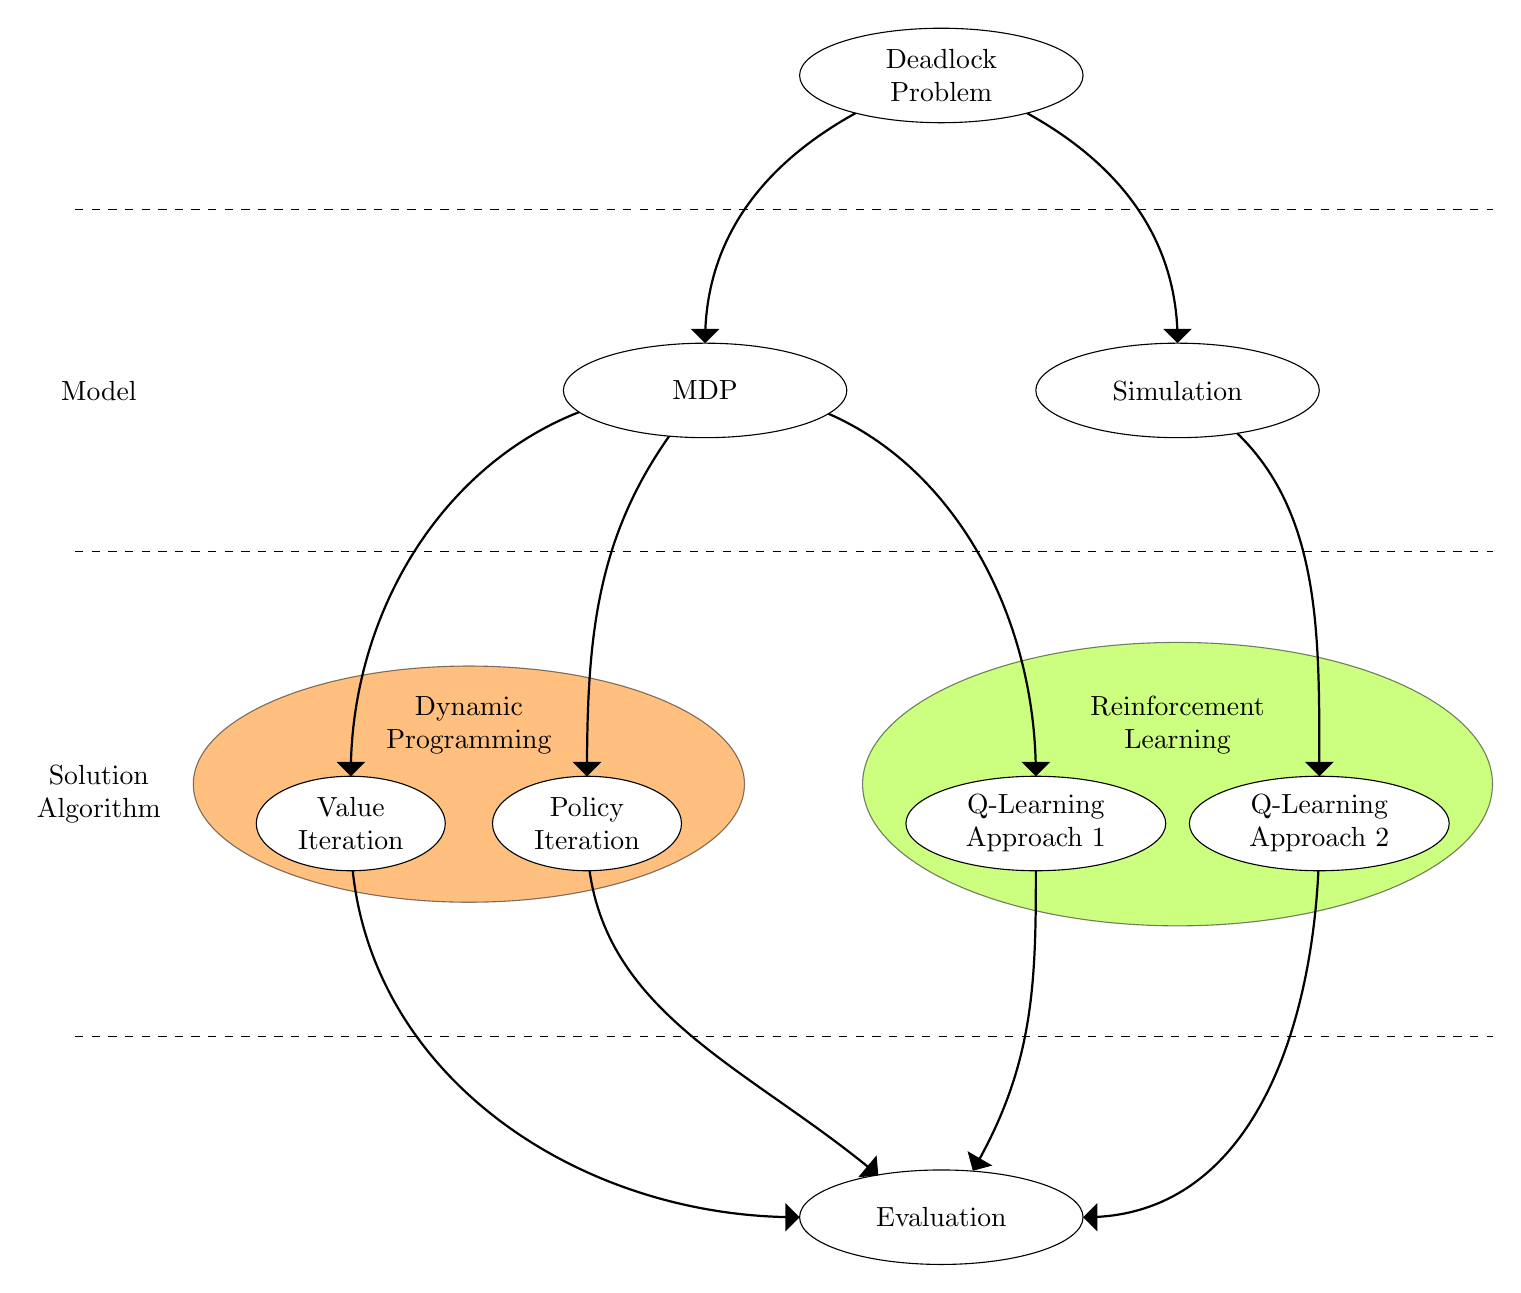
\begin{tikzpicture}


\node (mdp) at (-3, 1.5) {};
\node (sim) at (3, 1.5) {};
\node (vi) at (-7.5, -4) {};
\node (pi) at (-4.5, -4) {};
\node (ql2) at (4.8, -4) {};
\node (ql1) at (1.2, -4) {};
\node (prob) at (0, 5.5) {};




\draw[draw=black, fill=lime!80!green, opacity=0.5] (3, -3.5) ellipse (4 and 1.8);
\node[align=center] (rl) at (3, -2.75) {Reinforcement\\Learning};

\draw[draw=black, fill=orange, opacity=0.5] (-6, -3.5) ellipse (3.5 and 1.5);
\node[align=center] (dp) at (-6, -2.75) {Dynamic\\Programming};

\draw[draw=black, fill=white] (0, -9) ellipse (1.8 and 0.6);
\node (eval) at (0, -9) {Evaluation};



\draw (mdp) edge[out=180,in=90,- triangle 90,thick] (-7.5, -3.4);
\draw (mdp) edge[out=-130,in=90,- triangle 90,thick] (-4.5, -3.4);
\draw (mdp) edge[out=0,in=90,- triangle 90,thick] (1.2, -3.4);
\draw (sim) edge[out=-30,in=90,- triangle 90,thick] (4.8, -3.4);
\draw (prob) edge[out=-160,in=90,- triangle 90,thick] (-3, 2.1);
\draw (prob) edge[out=-20,in=90,- triangle 90,thick] (3, 2.1);


\draw[draw=black, fill=white] (-3, 1.5) ellipse (1.8 and 0.6);
\node at (-3, 1.5) {MDP};

\draw[draw=black, fill=white] (3, 1.5) ellipse (1.8 and 0.6);
\node at (3, 1.5) {Simulation};


\draw[draw=black, fill=white] (0, 5.5) ellipse (1.8 and 0.6);
\node[align=center] at (0, 5.5) {Deadlock\\Problem};


\draw (vi) edge[out=-90,in=180,- triangle 90,thick] (-1.8, -9);
\draw (pi) edge[out=-90,in=140,- triangle 90,thick] (-0.8, -8.47);
\draw (ql1) edge[out=-90,in=60,- triangle 90,thick] (0.4, -8.41);
\draw (ql2) edge[out=-90,in=0,- triangle 90,thick] (1.8, -9);

\draw[draw=black, fill=white] (-7.5, -4) ellipse (1.2 and 0.6);
\node[align=center] at (-7.5, -4) {Value\\Iteration};

\draw[draw=black, fill=white] (-4.5, -4) ellipse (1.2 and 0.6);
\node[align=center] at (-4.5, -4) {Policy\\Iteration};

\draw[draw=black, fill=white] (4.8, -4) ellipse (1.65 and 0.6);
\node[align=center] at (4.8, -4) {Q-Learning\\Approach 2};

\draw[draw=black, fill=white] (1.2, -4) ellipse (1.65 and 0.6);
\node[align=center] at (1.2, -4) {Q-Learning\\Approach 1};



\draw[dashed] (-11, 3.8) -- (7, 3.8);
\draw[dashed] (-11, -0.55) -- (7, -0.55);
\draw[dashed] (-11, -6.7) -- (7, -6.7);

\node[align=center] at (-10.7, 1.5) {Model};
\node[align=center] at (-10.7, -3.625) {Solution\\Algorithm};



\end{tikzpicture}

\end{document}